% Created 2024-03-11 ma 21:53
% Intended LaTeX compiler: pdflatex
\documentclass[bigger]{beamer}
\usepackage[utf8]{inputenc}
\usepackage[T1]{fontenc}
\usepackage{graphicx}
\usepackage{longtable}
\usepackage{wrapfig}
\usepackage{rotating}
\usepackage[normalem]{ulem}
\usepackage{amsmath}
\usepackage{amssymb}
\usepackage{capt-of}
\usepackage{hyperref}
\usepackage{graphicx}
\usepackage[export]{adjustbox}
\usepackage[round]{natbib}   % omit 'round' option if you prefer square brackets
\usetheme{default}
\author{Jeroen van Riel}
\date{March 2024}
\title{Traffic Scheduling}
\AtBeginSection[]{ \title{\secname}\author{}\date{} \begin{frame} \maketitle \end{frame}}
\hypersetup{
 pdfauthor={Jeroen van Riel},
 pdftitle={Traffic Scheduling},
 pdfkeywords={},
 pdfsubject={},
 pdfcreator={Emacs}, 
 pdflang={English}}
\begin{document}

\maketitle
\section{Single intersection}
\label{sec:orgde4894b}

\begin{frame}[label={sec:orgeed6ea9}]{Safe trajectories at isolated intersection}
\begin{figure}
  \centering
  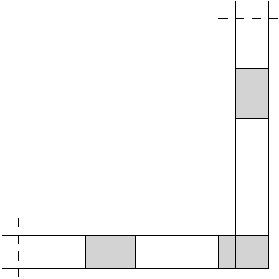
\includegraphics[width=0.3\textwidth]{../figures/miculescu_karaman.pdf}
\end{figure}

\begin{itemize}
\item trajectories \(x(t)\) satisfy contraints
\begin{subequations}
\begin{align}
0 \leq x'(t) \leq v_m \\
|x''(t)| \leq a_m
\end{align}
\end{subequations}
\item no collisions between vehicles

\item problem of optimal control is essentially reduced to finding an optimal policy in a two-queue polling system \cite{miculescuPollingsystemsbasedAutonomousVehicle2016}
\end{itemize}
\end{frame}
\begin{frame}[label={sec:org031a230}]{Two-queue polling system}
\begin{itemize}
\item two queues with customers arriving as Poisson(\(\lambda_i\)) process
\item single server alternates queues, location is \(u \in \{1,2\}\)
\item number of customers in queue \(i\) is denoted as \(x_i\)
\item service takes \(p\) time, switch takes \(s\) time
\end{itemize}

\vfill
\begin{figure}
  \centering
  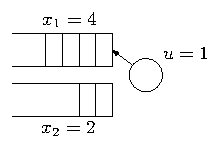
\includegraphics[width=0.5\textwidth]{../figures/polling.pdf}
\end{figure}
\end{frame}
\begin{frame}[label={sec:orgf5209bb}]{Semi-Markov Decision Process}
\begin{itemize}
\item Markov decision process with sojourn times \(\Upsilon_n\)
\item action space \(\mathcal{A} = \{P,S,I\}\)
\item state space \(\mathcal{S} = \{1,2\} \times \mathbb{N}^+ \times \mathbb{N}^+\)
\item serving and switching are non-preemptive, so skip arrivals while serving or switching
\end{itemize}

\vfill
\begin{figure}
  \centering
  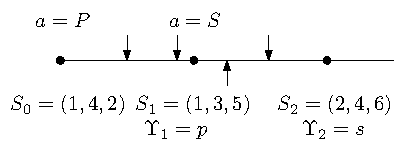
\includegraphics[width=0.9\textwidth]{../figures/polling_smdp.pdf}
\end{figure}
\end{frame}
\begin{frame}[label={sec:org498ec01}]{Semi-Markov Decision Process}
\begin{itemize}
\item holding costs for customers
\end{itemize}

\begin{align}
r(t) = -(x_1(t) + x_2(t))
\end{align}

\begin{itemize}
\item total discounted reward
\end{itemize}

\begin{align}
\phi_\beta = \mathbb{e} \left[ \int_0^\infty e^{-\beta t}r(t) dt \right]
\end{align}

\vfill
\begin{figure}
  \centering
  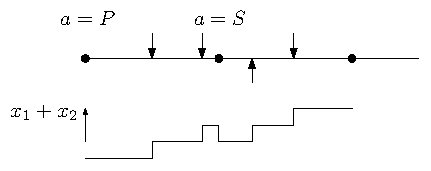
\includegraphics[width=0.9\textwidth]{../figures/polling_smdp_rewards.pdf}
\end{figure}
\end{frame}
\begin{frame}[label={sec:org44f88f6}]{Optimal policies}
\begin{itemize}
\item \cite{hofriOptimalControlTwo1987}
\begin{itemize}
\item theorem: there is an optimal exhaustive policy
\item conjecture: there is an optimal double-threshold policy
\end{itemize}

\item curse of modeling
\begin{itemize}
\item approximate the SMDP, then dynamic programming
\item Q-learning or similar model-free methods
\end{itemize}
\end{itemize}
\end{frame}
\begin{frame}[label={sec:org45b68b2}]{General arrival processes}
\begin{itemize}
\item extend the state space to include time since last arrival

\begin{align}
(u, x_1, x_2, \tau_1, \tau_2) \in \mathcal{S} = \{1,2\} \times \mathbb{N}^+ \times \mathbb{N}^+ \times \mathbb{R}^+ \times \mathbb{R}^+
\end{align}

\item explicitly discretize state space
\item parametric function approximation (neural net)
\end{itemize}
\end{frame}
\section{Knowledge of future arrivals}
\label{sec:orgda73aa2}

\begin{frame}[label={sec:orgb013001}]{Knowledge of future arrivals}
\begin{itemize}
\item extreme cases
\begin{itemize}
\item full knowledge (\(h=\infty\)) \(\implies\) planning
\item no knowledge (\(h=0\))
\end{itemize}
\end{itemize}

\vfill
\begin{figure}[t]
  \centering
  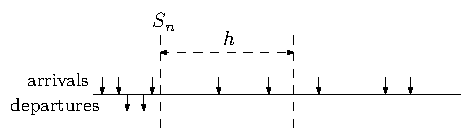
\includegraphics[width=0.9\textwidth]{../figures/horizon.pdf}
\end{figure}
\end{frame}
\begin{frame}[label={sec:org57a12fe}]{Full knowledge of future (planning)}
\begin{itemize}
\item general solution method via MILP formulation
\item \(r_j\) is arrival time
\item \(y_j\) is crossing time, \(C_j = y_j + p\) is completion time
\item \(o_{jl}\) is order of vehicles j and l (binary decision variable)
\item \(\mathcal{C}\) is set of precedence constraints
\item \(\bar{\mathcal{D}}\) is set of conflicts (between vehicles of distinct lanes)
\end{itemize}

\begin{subequations}
\begin{align}
  \text{minimize } & \sum_{j=1}^{n} C_{j} & \\
  \text{s.t. } & r_{j} \leq y_{j} & \text{ for all } j=1, \dots, n, \\
              & C_{j} \leq y_{l} & \text{ for all } (j,l) \in \mathcal{C}, \\
              & C_{j} + s \leq y_{l} + o_{jl}M  & \text{ for all } (j,l) \in \bar{\mathcal{D}}, \label{eq:disjunctive-constraints} \\
              & o_{jl} \in \{ 0, 1 \} & \text{ for all } (j,l) \in \bar{\mathcal{D}} .
\end{align}
\end{subequations}
\end{frame}
\begin{frame}[label={sec:orgc791cca}]{Full knowledge of future (planning)}
\begin{itemize}
\item example where waiting is necessary
\end{itemize}

\vfill
\begin{figure}[t]
  \centering
  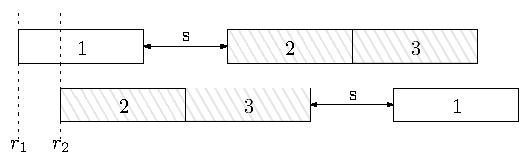
\includegraphics[width=0.65\textwidth]{../figures/123.pdf}
\end{figure}
\end{frame}
\begin{frame}[label={sec:org15d2608}]{No knowledge of future}
\begin{itemize}
\item polling system discussed at beginning
\item conjecture: waiting is required to obtain optimal policy
\item action space \(\mathcal{A} = \{P,S,I(\infty)\} \cup \{I(\delta) : \delta > 0\}\)
\end{itemize}
\end{frame}
\section{Multiple intersections}
\label{sec:orga680cc9}

\begin{frame}[label={sec:orga24ea9f}]{Job Shop}
\begin{itemize}
\item extension of MILP to multiple intersections is trivial
\item similar to job-shop machine scheduling
\item no guarantees for existence of safe trajectories
\item finite buffer space between intersections
\end{itemize}
\end{frame}
\begin{frame}[label={sec:org93d50de}]{End-to-end methods}
\begin{itemize}
\item define very general policy space
\item use model-free reinforcement learning to find policies
\end{itemize}
\end{frame}
\begin{frame}[label={sec:org2727cf1}]{References}
\begingroup
\renewcommand{\section}[2]{}
\bibliography{../references}
\bibliographystyle{plainnat}
\endgroup

\(\;\)
\end{frame}
\end{document}
